\section{Joint representation learning}
\label{sec:ch6:joint}

In many problems, our network might be more than just the information contained in its adjacency matrix (called its \textit{network topology}, or its collection of nodes and edges). If we were investigating a social network, we might have access to extra information about each person -- their gender, for instance, or their age. If we were investigating a brain network, we might have information about the physical location of neurons, or some notion of how big a brain region is. When we embed a network, it seems like we should be able to use these extra bits of information - called the ``features'' or ``covariates'' of the nodes in the network - to somehow improve our analysis. The techniques and tools that we'll explore in this section use both the covariates and the topology of a network to create and learn from new representations of the network. Because they jointly use both the topology of the network and its extra covariate information, these techniques and tools are called joint representation learning.

There are two primary reasons that we might want to explore using node covariates in addition to topological structure. First, they might improve our standard embedding algorithms, like Laplacian and Adjacency Spectral Embedding. For example, if the latent structure of the covariates of a network lines up with the latent structure of its topology, then we might be able to reduce noise when we embed, even if the communities in our network don't overlap perfectly with the communities in our covariates. Second, figuring out what the clusters of an embedding actually mean can sometimes be difficult and covariates create a natural structure in our network that we can explore. Covariate information in brain networks telling we where in the brain each node is, for instance, might let us better understand the types of characteristics that distinguish between different brain regions.

In this section, we'll explore different ways to learn from our data when we have access to the covariates of a network in addition to its topological structure. we'll explore \textit{Covariate-Assisted Spectral Embedding} (\texttt{case}), a variation on Spectral Embedding developed by \cite{Binkiewicz2017Jun}. In \texttt{case}, instead of embedding just the adjacency matrix or its Laplacian, we will combine the Laplacian and our covariates into a new matrix and embed that.

\begin{floatingbox}[h]\caption{School network example}
A good way to illustrate how using covariates might help us is to use a model in which some of our community information is in the covariates and some is in our topology. Let's imagine we have a network of $N=200$ nodes representing wikipedia pages for two complementary fields; computer science and statistics. A pair of wikipedia pages have an edge if both of the wikipedia pages link to one another. 

Unfortunately in our network, there is an extremely strong and prominent core: the top $50$ computer science wikipedia pages and the top $50$ statistics wikipedia pages tend to overwhelmingly cross-link to one another, and do not tend to link to the peripheral, more specialized, pages nearly as much.

When you attempt to embed this network via a strategy you have learned already like \texttt{ase}, you will likely be able to yield an embedding differentiate the strong core very easily from the periphery, but you will struggle to parse out the ``subject-matter specific'' signal of retaining the differences between computer science and statistics articles.

Fortunately, you also have another piece of information: whether a given page cites each of the twenty most influential statisticians of all time. This is a simple indicator for each statistician; a value of $1$ is recorded for page $i$ and statistician $k$ if statistician $k$ is cited by page $i$.
\end{floatingbox}

Let's first generate the network data for the wikipedia pages:

\begin{lstlisting}[style=python]
import numpy as np


n = 200  # total number of nodes
# first two communities are the ``core'' pages for statistics
# and computer science, and second two are the ``peripheral'' pages
# for statistics and computer science.
B = np.array([[.4, .3, .05, .05],[.3, .4, .05, .05],[.05, .05, .05, .02],[.05, .05, .02, .05]])

# make your stochastic block model
A, labels = sbm([n // 4, n // 4, n // 4, n // 4], B, return_labels=True)
# generate labels for core/periphery
co_per_labels = ["Core" for i in range(n // 2)] + ["Periphery" for i in range(n // 2)]
# generate labels for statistics/CS
st_cs_labels = ["Stat" for i in range(n // 4)] + ["CS" for i in range(n // 4)] + \
            ["Stat" for i in range(n // 4)] + ["CS" for i in range(n // 4)]
\end{lstlisting}

The network is shown in Figure \ref{fig:ch6:casc:casc_net}(A). We show the results of a \texttt{lse} of the network into two dimensions in Figure \ref{fig:ch6:casc:casc_net}(B). Note that embedding this network, we can only do a decent job of distinguishing the core nodes (from both CS and Statistics) from the periphery nodes (from both CS and Statistics), but we cannot differentiate between the two subject materials.

\begin{figure}[h]
    \centering
    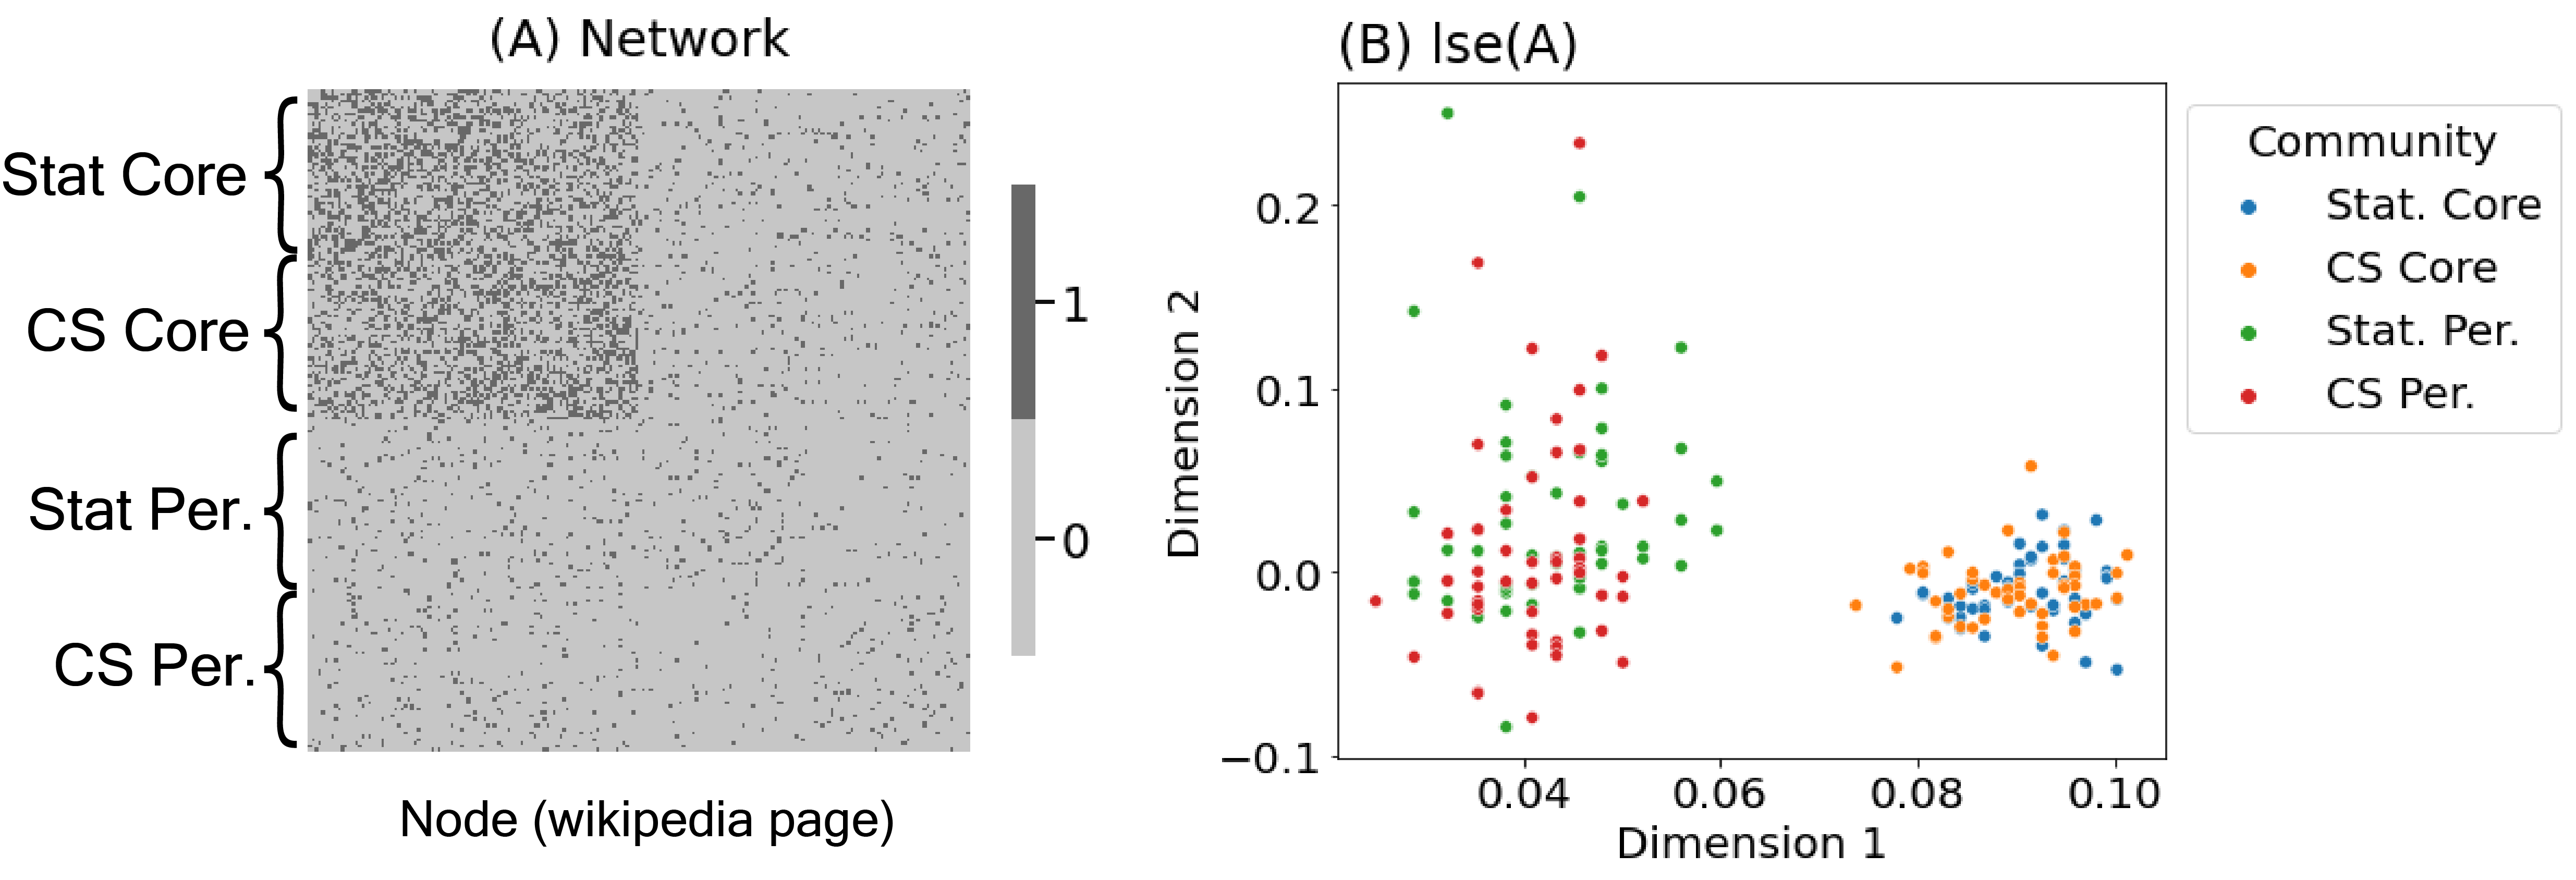
\includegraphics[width=\linewidth]{representations/ch6/Images/casc_net.png}
    \caption[\texttt{CASC} network]{\textbf{(A)} the wikipedia network, \textbf{(B)} a \texttt{lse} of the wikipedia network.}
    \label{fig:ch6:casc:casc_net}
\end{figure}

Next, we'll focus on generating the covariates associated with each node. We have a simple binary indicator for each page, indicating whether any of our twenty influential statisticians are cited. For statistics pages, there is a $50\%$ change that each of the twenty statisticians are cited. However, for computer science pages, there is only a $5\%$ chance that any of the three statisticians are cited. We can generate these covariates like this, using \texttt{numpy}:

\begin{lstlisting}[style=python]
trial = []
for label in st_cs_labels:
    if "Stat." in label:
        # if the page is a statistics page, there is a 40% chance
        # of citing each of the scholars
        trial.append(np.random.binomial(1, 0.5, size=20))
    else:
        # if the page is a CS page, there is a 5% chance of citing
        # each of the scholars
        trial.append(np.random.binomial(1, 0.05, size=20))
Y = np.vstack(trial)
\end{lstlisting}

The covariate matrix is plotted in Figure \ref{fig:ch6:casc:cov_repr}(A). Next, we perform a \texttt{pca} with the covariates, to determine whether we could learn the four communities (core and periphery of statistics and computer science) using only the covariate data:

\begin{lstlisting}[style=python]
def embed(X, d=2):
    """
    A function to embed a matrix.
    """
    Lambda, V = np.linalg.eig(X)
    return V[:, 0:d] @ np.diag(np.sqrt(np.abs(Lambda[0:d])))

def pca(X, d=2):
    """
    A function to perform a pca on a data matrix.
    """
    X_centered = X - np.mean(X, axis=0)
    return embed(X_centered @ X_centered.T, d=d)

Y_embedded = pca(Y, d=2)
\end{lstlisting}
We plot the resulting embedding in Figure \ref{fig:ch6:casc:cov_repr}(B). note that this time, we have excellent separation of the statistics and computer science pages, but we cannot differentiate the core from the periphery.

\begin{figure}[h]
    \centering
    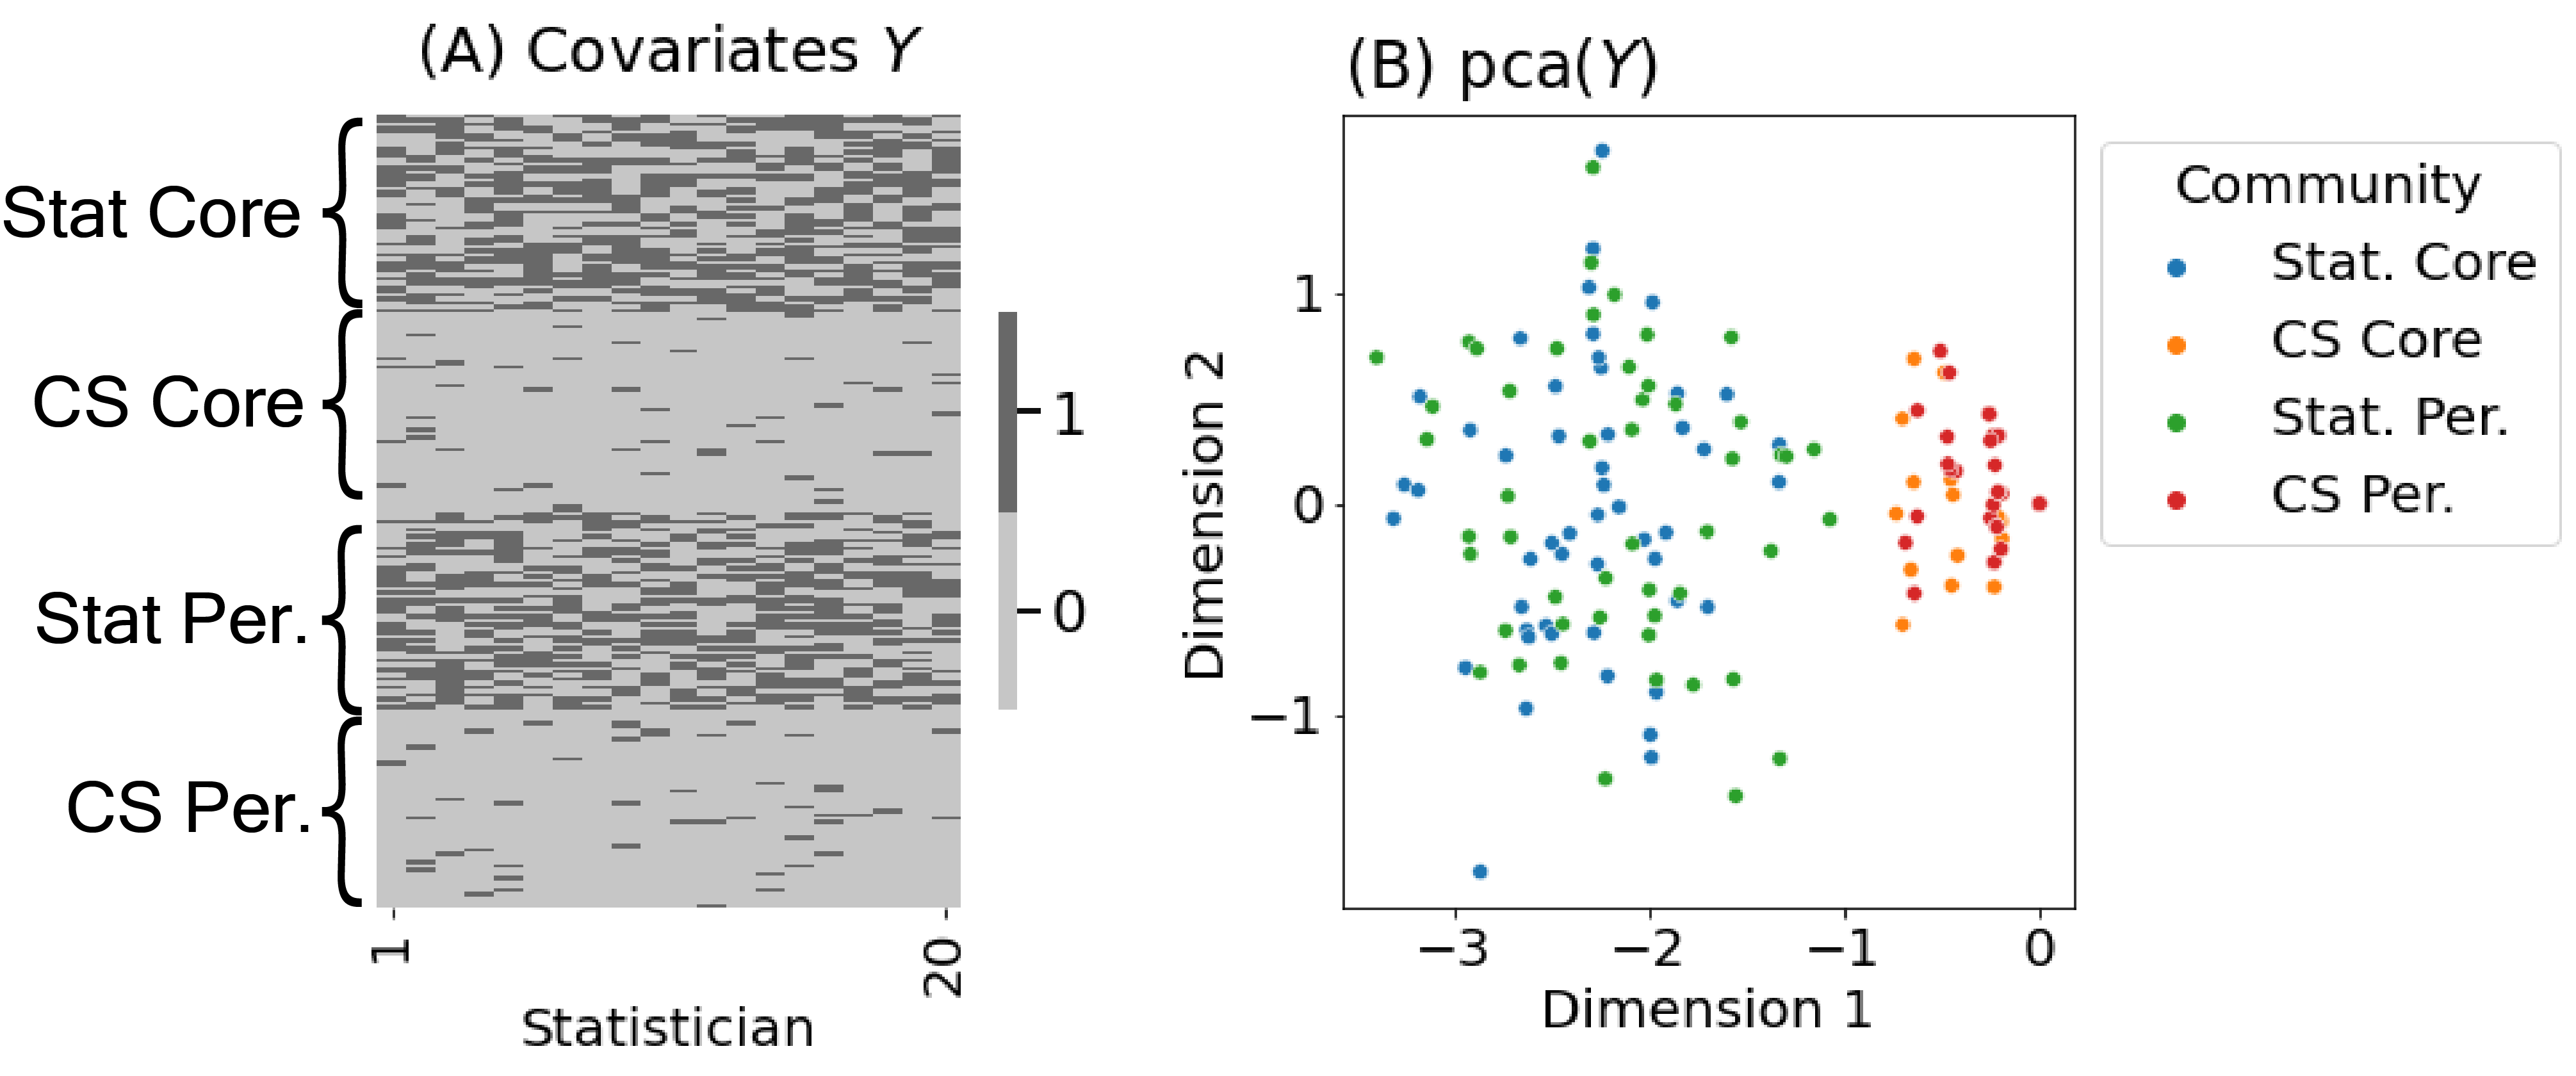
\includegraphics[width=\linewidth]{representations/ch6/Images/casc_covs.png}
    \caption[\texttt{pca} of covariates]{\textbf{(A)} the covariates associated with each wikipedia page, \textbf{(B)} a \texttt{pca} of the covariate data.}
    \label{fig:ch6:casc:cov_repr}
\end{figure}

\subsection{Covariate-Assisted Spectral Embedding}

\textit{Covariate-Assisted Spectral Embedding}, or \texttt{case}, is a simple way of combining our network and our covariates into a single model. In the most straightforward version of \texttt{case}, we take a weighted combination of the network's Laplacian $L$ and a similarity matrix for our covariates, $YY^\top$. 

\begin{floatingbox}\caption{Connections to Principal Components Analysis (\texttt{pca})}
\label{box:ch6:casc:pca}
If you have studied machine learning previously, this matrix should look familiar to you.

Note that the rows of the matrix $Y$, denoted by $\vec y_i$, are each $20$-dimensional vectors, where each entry has a value of $0$ of $1$. The matrix product $YY^\top$ has entries:
\begin{align*}
    (YY^\top)_{ij} = \vec y_i^\top \vec y_j = \sum_{k = 1}^{20} y_{ik}y_{jk}.
\end{align*}
In this case, since the values of our covariate matrix can take only $0$s and $1$s, this basically just counts up the number of times wikipedia page $i$ and wikipedia page $j$ both cite scholar $k$. In this sense, you can conceptualize the uncentered, un-rescaled covariance matrix $YY^\top$ as giving a degree of ``similarity'' in the covariates for each of our nodes. 

Much like \texttt{ase} exploits latent behaviors in the adjacency matrix to determine an appropriate embedding, a \texttt{pca} exploits latent behaviors in the covariances of our data matrix (here, our covariates, $Y$) to embed a given dataset. Typically, \texttt{pca} would spectrally embed the centered and scaled covariance matrix:
\begin{align*}
    \frac{1}{n - 1}\left(Y - \vec \mu_y\right)\left(Y - \vec \mu_y\right)^\top
\end{align*}
This is distinct from the procedure that we are using here, because we will not typically take the centering nor the scaling steps (but, we certainly could).
\end{floatingbox}

Let's take a look at what the network Laplacian and the covariate similarity matrix $YY^\top$ look like here:

\begin{lstlisting}[style=python]
from graspologic.utils import to_laplacian

# compute the network Laplacian
L_wiki = to_laplacian(A, form="DAD")
# log transform, strictly for visualization purposes
L_wiki_logxfm = np.log(L_wiki + np.min(L_wiki[L_wiki > 0])/np.exp(1))

# compute the node similarity matrix
Y_sim = Y @ Y.T
\end{lstlisting}

The network Laplacian and the node similarity matrix are shown in Figure \ref{fig:ch6:casc:casc_inputs}. Note that we used the log-transforming strategy from Section \ref{fig:ch4:log_xfm} to visualize the log-transformed Laplacian after adding a suitably small offset $\epsilon$, as many of the network weights were extremely small, so the color scale was not particularly informative on the Laplacian itself (try plotting it yourself).

\begin{figure}
    \centering
    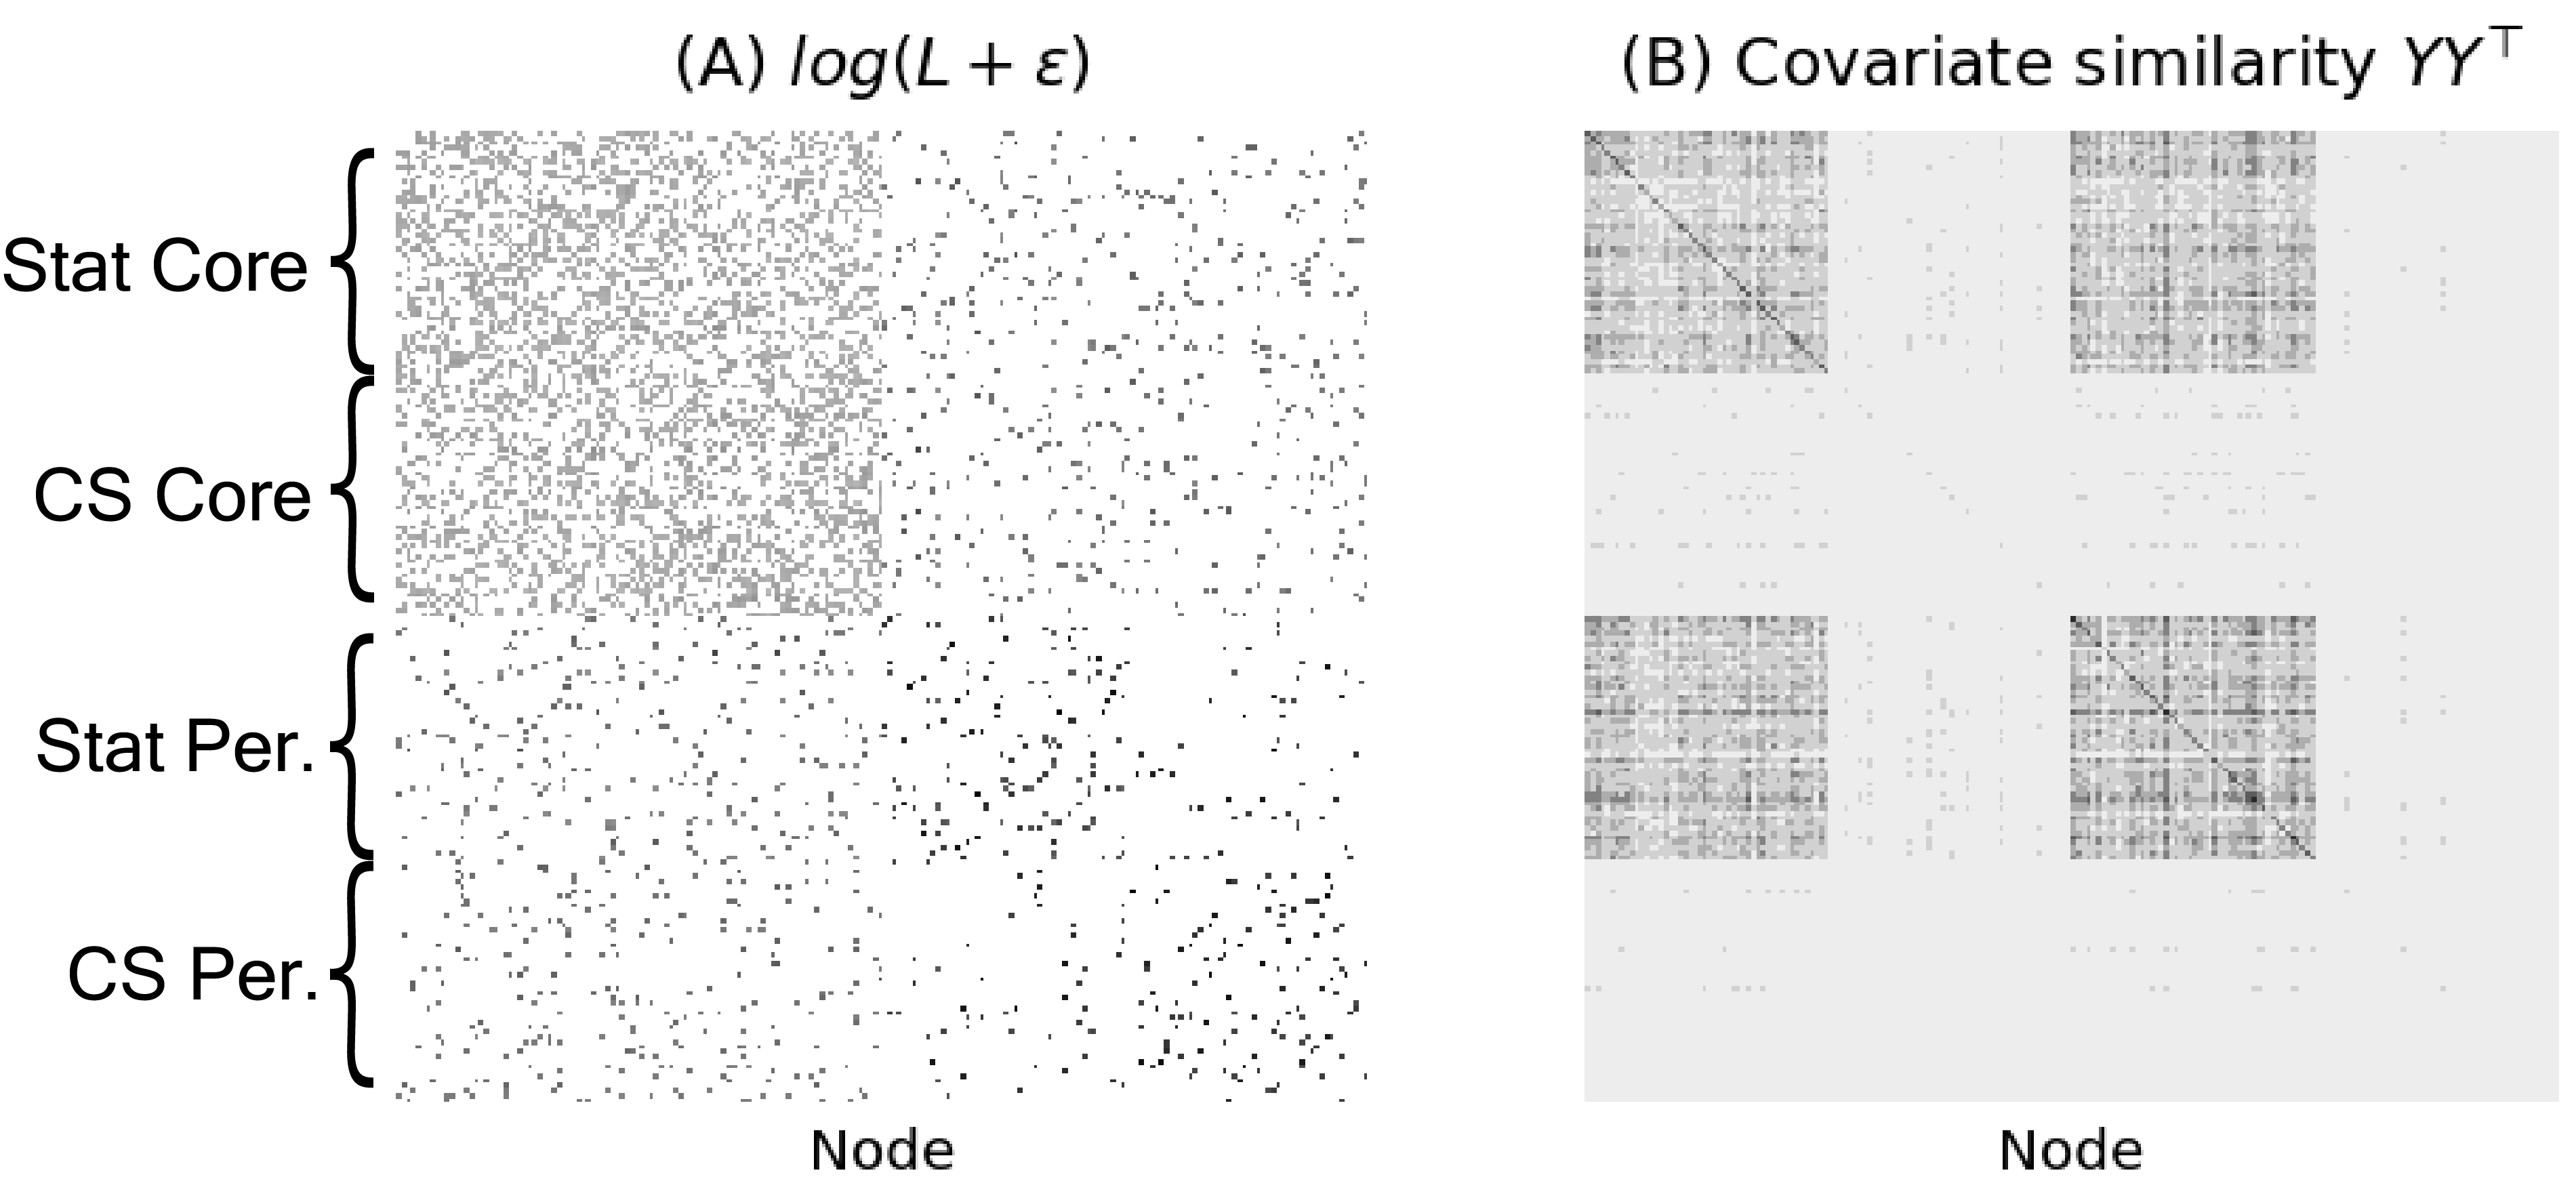
\includegraphics[width=\linewidth]{representations/ch6/Images/casc_inputs.png}
    \caption[inputs to \texttt{case}]{\textbf{(A)} a visualization of the log-transformed network Laplacian, and \textbf{(B)} the covariate similarity matrix.}
    \label{fig:ch6:casc:casc_inputs}
\end{figure}

Note that each embedding appears to preserve disparate properties about the underlying network: the topology of the network, reflected in the network Laplacian, conveys the topological disparities between the core and peripheral pages in our network. On the other hand, the covariate metadata that we have associated with each node in the network conveys the content disparities between the statistics and computer science nodes in the network. 

\paragraph*{Combining information from the network topology and the covariates}

The matrix that is spectrally embedded through \texttt{case} is a linear combination of the network Laplacian $L$ and the covariate similarity matrix $YY^\top$. It is typically represented like this:
\begin{align*}
    L + \alpha YY^\top.
\end{align*}
The weight $\alpha$ is a hyper-parameter to the \texttt{case} technique, in that it is a parameter that we will often want to select with respect to a downstream task of interest. 

\begin{lstlisting}[style=python]
from graspologic.embed import AdjacencySpectralEmbed

def case(A, Y, weight=0, d=2, tau=0):
    """
    A function for performing case.
    """
    # compute the laplacian
    L = to_laplacian(A, form="R-DAD", regularizer=tau)
    YYt = Y @ Y.T
    return AdjacencySpectralEmbed(n_components=2)(L + weight*YYt)

embedded = case(A, Y, weight=.002)
\end{lstlisting}

For instance, if we had a high-level goal of producing an embedding which preserved both topological properties of the network (such as the core and peripheral components) as well as covariate-derived properties of the network (such as statistics and computer science components), a heuristic might be to try numerous weights $\alpha$, and evaluate the resulting embeddings for each choice of $\alpha$. A suitable choice of $\alpha$ would be a choice in which the community groupings are preserved.

\begin{figure}[h]
    \centering
    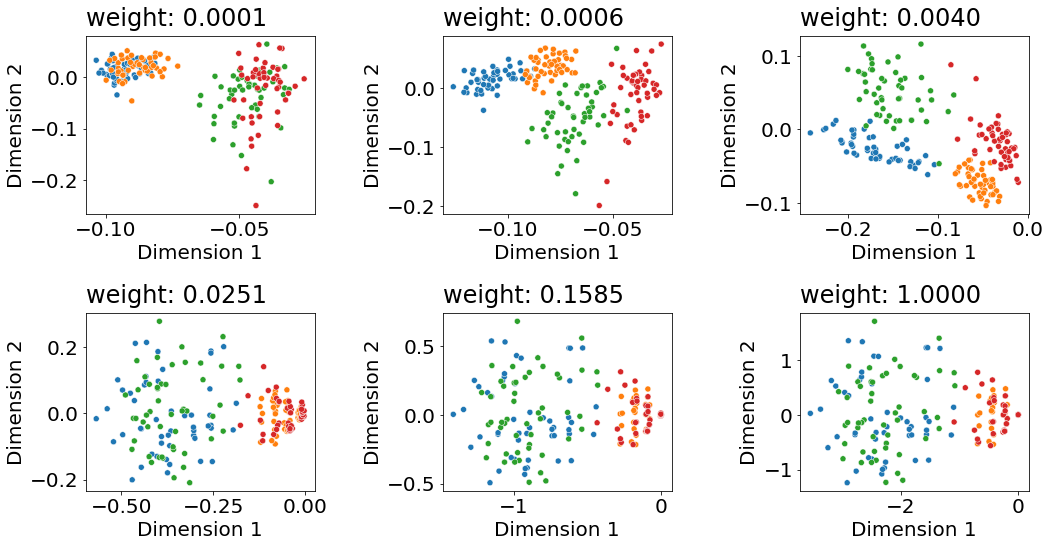
\includegraphics[width=\linewidth]{representations/ch6/Images/case_outputs.png}
    \caption[CASE embedding example]{The network embedding using both the network topology and the node covariates, for different choices of $\alpha$.}
    \label{fig:ch6:casc:casc_out}
\end{figure}
Figure \ref{fig:ch6:casc:casc_out} explores various network embeddings with different choices of $\alpha$. Note that for low choices of $\alpha$, the embedding resembles that of the topology only \texttt{lse} in Figure \ref{fig:ch6:casc:casc_net}(B). For large choices of $\alpha$, the embedding closely resembles that of the covariate-only embedding in Figure \ref{fig:ch6:casc:cov_repr}(B). For the intermediate choices, such as $\alpha = .0006$ or $\alpha = .004$, the embedding appears to leverage information across both the covariates and the network topology, and both the core/periphery and subject matter (statistics/computer science) structures are preserved.

\subsubsection{Automatic weight selection}

In general, it is ideal to perform joint representation learning with an approach like \texttt{case} with a downstream machine learning task in mind. This is because the weight selection procedure of \texttt{case} is a search over hyperparameters, and it is difficult to determine what an appropriate hyperparameter choice is without any way to evaluate your hyperparameter. For instance, in the evaluation above, we determined ``ideal'' weight selections to be on the basis of how well different weights established community structure for known communities. We could make such a search more quantitative by incorporating a procedure which quantifies ``community separation'' between groups of nodes.

While we cannot automatically determine an ``ideal'' weight in terms of an arbitrary downstream task that you might have, we can take principled steps to ensure that the two components of \texttt{case} (the normalized Laplacian and the covariate similarity matrix) are contributing relatively equally to the embedding process.

When you embed symmetric matrices, keep in mind that the actual points you’re plotting are the components of the eigenvectors with the biggest eigenvalues. When you embed into two-dimensional space, for instance, the $x$-axis values of your points are the components of the eigenvector with the biggest eigenvalue, and the $y$-axis values are the components of the eigenvector with the second-biggest eigenvalue. This means that you should probably be thinking about how much information the Laplacian and contributes to the biggest eigenvalue/eigenvector pairs.

Thinking about this more, if you have a small weight, $YY^\top$ will contribute only a small amount to the biggest eigenvalue/vector pair. If you have a large weight, $YY^\top$ will contribute a large amount to the biggest eigenvalue/vector pair. A roughly prudent starting point for your embedding, therefore, might be the ratio of the biggest eigenvalue of $L$ and the biggest eigenvalue of $YY^\top$:

\begin{align*}
\alpha_0 = \frac{\lambda_1 (L)}{\lambda_1 (YY^\top)}    
\end{align*}

The \texttt{case} procedure can be automated in \texttt{graspologic}, with:

\begin{lstlisting}[style=python]
from graspologic.embed import CovariateAssistedEmbed as case

embedding = case(alpha=None, n_components=2).fit_transform(A, covariates=Y)
\end{lstlisting}
To specify a specific weight, you can do so with the \texttt{alpha} parameter.

\subsection{Considerations for positive semi-definiteness}

As we will see in Section \ref{sec:ch6:dimest:grdpg}, most of the techniques discussed thus far theoretically operate well under a relatively homogeneous setting captured by the gRDPG. This setting extends the intuition of what we have discussed (which, conceptually, we tended to stick to the positive semi-definite case) to the non positive semi-definite case. 

\texttt{case} operates a bit on its own compared to the other algorithms described in this section, and does not quite fall into the same theoretical framework (despite sharing many conceptual and intuitive similarities). In the situation where you have reason to believe that the random network underlying your experiment is not positive semi-definite, such as if you are able to identify a disassortative block structure (from Section \ref{sec:ch5:psd_block}), you can alter your Laplacian to be positive semi-definite by simply instead embedding $LL + \alpha YY^\top$. This can be done in \texttt{graspologic} with:

\begin{lstlisting}[style=python]
embedding = case(assortative=False, n_components=2).fit_transform(A, covariates=Y)
\end{lstlisting}

When you are not sure whether the structure of your network supports positive semi-definite or non positive semi-definite structure in the underlying random network, the authors advise \cite{Binkiewicz2017Jun} that non-assortative \texttt{case} tends to perform nearly as well under assortative structures, and far better under non-assortative structures.

\subsection{Extensions of \texttt{case}}

In this section, we introduced a relatively simple technique for augmenting our typical \texttt{lse} algorithm for the case where we had node-specific covariate information. We accomplished this via a matrix $YY^\top$, which we combined (with a suitable weight parameter) with our Laplacian.

That said, an extension that you might have is to consider other possible similarity functions (other than simply the inner product $\vec y_i^\top \vec y_j$) that you might use for covariate assisted embedding techniques. For instance, \texttt{graspologic} also allows centering and scaling steps to be taken, in much the same vein as the typical pre-processing steps for \texttt{pca}. You could further generalize this strategy to other similarity functions entirely. In your work, you may be motivated to define other similarity criteria that go beyond this approach that was originally used in \cite{Binkiewicz2017Jun} to devise new approaches for covariate-assisted spectral embeddings.


\newpage